%\documentclass[12pt,notitlepage]{article}
\documentclass[a4paper,12pt]{article}
\usepackage[utf8]{inputenc}
\usepackage{graphicx}
\usepackage{verbatim}
\usepackage{amsthm}
\usepackage{amssymb}
\usepackage{pdfpages}
\usepackage{amsmath}
\usepackage{tikzsymbols}
\usetikzlibrary{arrows}
\usetikzlibrary{3d}
\newcommand{\midarrow}{\tikz \draw[-triangle 90] (0,0) -- +(.1,0);}
\pgfdeclarelayer{bg}    % declare background layer
\pgfsetlayers{bg,main}  % set the order of the layers (main is the standard layer)
\usepackage{mwe}
\usetikzlibrary{decorations.pathreplacing}
\usetikzlibrary{shapes}
\usepackage{mathtools}
\usepackage{enumitem}
\DeclarePairedDelimiter\ceil{\lceil}{\rceil}
\DeclarePairedDelimiter\floor{\lfloor}{\rfloor}
\usepackage{subcaption}

\usepackage{hyperref}
%\usepackage[T1]{fontenc}
\usepackage{url}
\usepackage{lipsum}
\usepackage{array}
\usepackage{multirow}
\usepackage{float}
\usepackage{lscape}
\usepackage{colortbl}
\newcolumntype{P}[1]{>{\centering\arraybackslash}p{#1}}
\usepackage[nottoc,numbib]{tocbibind}
\usepackage{fancyhdr}
\usepackage{hhline}
\usepackage[printonlyused]{acronym}
\usepackage{footmisc}

%\usepackage{txfonts}
\usepackage{lipsum,etoolbox}% http://ctan.org/pkg/{lipsum,etoolbox}
\usepackage{caption}
\usepackage{subcaption}
\usepackage{setspace}

\usepackage{algorithm}
\usepackage[noend]{algpseudocode}

\makeatletter
\def\BState{\State\hskip-\ALG@thistlm}
\makeatother

\usepackage{minted}

\definecolor{black}{RGB}{0,0,0}

\usepackage{fancyvrb}

\usepackage{geometry}
\geometry{
	a4paper,
	total={170mm,257mm},
	right=3cm,
	left=3cm,
	top=3cm,
	bottom=3cm
}



\makeatletter
\DeclareRobustCommand{\rvdots}{%
	\vbox{
		\baselineskip4\p@\lineskiplimit\z@
		\kern-\p@
		\hbox{.}\hbox{.}\hbox{.}
}}
\makeatother
\usepackage{titlesec}
\usepackage{hyperref}
\titleclass{\subsubsubsection}{straight}[\subsection]

\newcounter{subsubsubsection}[subsubsection]
\renewcommand\thesubsubsubsection{\thesubsubsection.\arabic{subsubsubsection}}
\renewcommand\theparagraph{\thesubsubsubsection.\arabic{paragraph}} % optional; useful if paragraphs are to be numbered

\titleformat{\subsubsubsection}
{\normalfont\normalsize\bfseries}{\thesubsubsubsection}{1em}{}
\titlespacing*{\subsubsubsection}
{0pt}{3.25ex plus 1ex minus .2ex}{1.5ex plus .2ex}

\makeatletter
\renewcommand\paragraph{\@startsection{paragraph}{5}{\z@}%
	{3.25ex \@plus1ex \@minus.2ex}%
	{-1em}%
	{\normalfont\normalsize\bfseries}}
\renewcommand\subparagraph{\@startsection{subparagraph}{6}{\parindent}%
	{3.25ex \@plus1ex \@minus .2ex}%
	{-1em}%
	{\normalfont\normalsize\bfseries}}
\def\toclevel@subsubsubsection{4}
\def\toclevel@paragraph{5}
\def\toclevel@paragraph{6}
\def\l@subsubsubsection{\@dottedtocline{4}{7em}{4em}}
\def\l@paragraph{\@dottedtocline{5}{10em}{5em}}
\def\l@subparagraph{\@dottedtocline{6}{14em}{6em}}
\makeatother
\newcommand*\circled[1]{\tikz[baseline=(char.base)]{
		\node[shape=circle,draw,inner sep=2pt] (char) {#1};}}


\setcounter{secnumdepth}{4}
\setcounter{tocdepth}{4}
\newcommand{\und}{\underline{\hspace{.10in}}}
\begin{document}
	\begin{titlepage}
		\begin{center}
			\vspace*{9em}
			\Huge 
			MH4921\\ Supervised Independent Study II\\
			\vspace*{4em}
			\LARGE
			\textbf{Linux Virtual Private Network (VPN) Lab}\\		
			\vspace{4em}
			\textbf{Brandon Goh Wen Heng}\\
			\vspace*{4em}
			Academic Year 2018/19
			\vfill
		\end{center}
	\end{titlepage}
	
	\pagenumbering{roman}
	\tableofcontents
	\newpage
	\pagenumbering{arabic}
	\section{Introduction}
	Organisation, Internet Service Providers (ISPs) and countries often block users from accessing certain external sites through what is known as egress filtering. This is used within organisations to reduce distractions, countries may make use of it to censor foreign web sites. However, these firewalls can easily be bypassed and there are multiple services/applications that aid in the circumvention.\\\\The most common technology that is used to bypass these egress filtering are Virtual Private Networks (VPNs). VPNs are also commonly available on smartphone devices to help bypass these egress firewalls.
	\section{Overview}
	This lab will focus on how the VPN works and how it can be used to bypass egress firewalls. A VPN usually depends on two components, IP tunnelling and encryption. Tunnelling is crucial in helping to bypass these firewalls while the encryption helps to protect the content that is being transmitted through the VPN tunnel. For simplicity, encryption is not in the scope of this lab.
	\section{Exploration}
	Implementing a simple VPN for \texttt{Linux} is not trivial and is broken into multiple segments, with detailed observations for each step in the process. By setting up the VPN, a tunnel is established between two systems. When system A is behind a firewall and wants to access restricted resources, it will be blocked by egress filtering. Therefore, the packets are routed through to system B where it will send the packets out to the Internet. Similarly, the response from the Internet will be routed through to system B before sending it back to system A via the tunnel. This is how the VPN helps system A to bypass the firewall.
	\subsection{Virtual Machine (VM) Setup}
	\subsubsection{VM Configuration}
	Two VMs are required for this lab. VM1 is behind a firewall while VM2 is outside the firewall. The objective is to help VM1 bypass the firewall so it is able to access blocked sites on the Internet.\\\\VM1 and VM2 are connected to a separate NAT adapter, so both can access the Internet using the corresponding NAT servers. To emulate the Internet, where both VM1 and VM2 can communicate to each other, both VMs are connected to a host-only network adapter. This network emulates the facilitation of communication between the two VMs. The network setup is depicted in figure 1 for easier reference.
	
	\begin{figure}[H]
		\centering
		\begin{tikzpicture}			
		\draw[fill=red!10] (-5.25,2.15) rectangle (-3.95,1.25);
		\draw (-5.4,2.3) rectangle (-3.8,1.1);
		\draw (-4.6,0.3) node[text width=3cm, align=center]{NAT Server\\10.0.2.1};
		
		\draw(-2.3,1.65) node{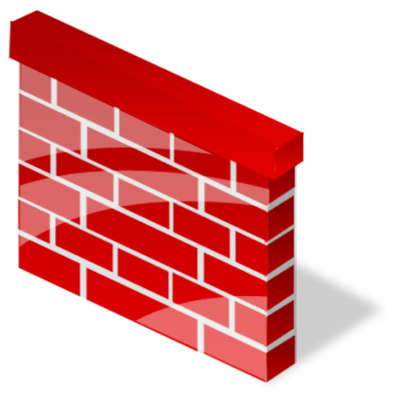
\includegraphics[width=0.10\linewidth,height=0.18\linewidth]{firewall.png}};
		\draw(-2.3,0.05) node {Firewall};
		\node[cloud, draw,cloud puffs=12,cloud puff arc=160, aspect=3, inner ysep=0.1cm, inner xsep=0.1cm, text width=1.8cm,align=center] at (0.3,1.69)  {Internet} ;
		
		\draw[fill=red!10] (3.45,2.15) rectangle (4.75,1.25);
		\draw (3.3,2.3) rectangle (4.9,1.1);
		\draw (4.1 ,0.3) node[text width=3cm, align=center]{NAT Server\\10.0.3.1};	
		
		\draw[fill=yellow!10] (-3.1,-1.35) rectangle (-1.8,-2.25);
		\draw (-3.25,-1.2) rectangle (-1.65,-2.4);
		\draw (-2.05,-2.4) rectangle (-2.85,-2.9);
		\draw (-3.05,-2.75) -- (-3.45,-3.1);
		\draw (-1.85,-2.75) -- (-1.45,-3.1);
		\draw (-3.45,-3.1) -- (-1.45,-3.1);
		\draw (-3.05,-2.75) -- (-2.85,-2.75);
		\draw (-1.85,-2.75) -- (-2.05,-2.75);
		\draw (-2.45,-3.8) node[text width=3cm,align=center]{VM1\\192.168.10.5};
		
		\draw[fill=yellow!10] (1,-1.35) rectangle (2.3,-2.25);
		\draw (0.85,-1.2) rectangle (2.45,-2.4);
		\draw (2.05,-2.4) rectangle (1.25,-2.9);
		\draw (1.05,-2.75) -- (0.65,-3.1);
		\draw (2.25,-2.75) -- (2.65,-3.1);
		\draw (0.65,-3.1) -- (2.65,-3.1);
		\draw (1.05,-2.75) -- (1.25,-2.75);
		\draw (2.25,-2.75) -- (2.05,-2.75);
		\draw (1.65,-3.8) node[text width=3cm,align=center]{VM2\\192.168.10.6};
		
		\draw(-3.8,1.7) -- (-2.98,1.7);
		\draw(-1.95,1.7) -- (-1.17,1.7);
		\draw(3.3,1.7) -- (1.76,1.7);
		
		\draw (-5.4,1.7) -- (-6.5,1.7);
		\draw (-3.25,-1.8) -- (-6.5,-1.8);
		\draw (-6.5,-2.3) --node[text width=4.5cm,align=center,rotate=90]{NAT - Network\\(10.0.2.0/24)} (-6.5,2.2);
		
		\draw(4.9,1.7)--(6,1.7);
		\draw(2.45,-1.8) -- (6,-1.8);
		\draw(6,-2.3) --node[text width=4.5cm,align=center,rotate=-90]{NAT - Network\\(10.0.3.0/24)} (6,2.2);
		
		\draw (-1.65,-1.8) -- (-0.8,-1.8);
		\draw (0.85,-1.8) -- (0,-1.8);
		\draw (-0.8,-1.8) -- (-0.8,-4.8);
		\draw (0,-1.8) -- (0,-4.8);
		\draw (-4,-4.8)--(3.2,-4.8);
		\draw (-0.4,-4.8) node[text width=7.2cm,align=center,yshift=-0.6cm]{Host-only Network\\(192.168.10.0/24)};
		
		
		\end{tikzpicture}
		\caption{Network Topology}
		\label{fig:Networksetup}
	\end{figure}
	\iffalse
	\subsubsection{Firewall Configuration}
	To emulate a corporate/academic environment, we use a packet firewall \texttt{ufw} to prevent any unwanted traffic exiting/entering the internal network. The following ports between 1--1023 are blocked from accessing any traffic (common system ports).
	\begin{enumerate}
		\itemsep0em 
		\item 20 -- File Transfer Protocol (FTP) data transfer
		\item 21 -- FTP control
		\item 22 -- Secure Shell (SSH)
		\item 23 -- Telnet
		\item 80 -- HyperText Transfer Protocol (HTTP) (Unsecured websites)
		\item 443 -- HyperText Transfer Protocol over TLS/SSL (HTTPS) (Secured websites)
		\item 514 -- Remote Shell
		\item 989 -- File Transfer Protocol over TLS/SSL (FTPS) data transfer
		\item 990 -- FTPS control
		\item 992 -- Telnet protocol over TLS/SSL
	\end{enumerate}
	\begin{figure}[H]
		\centering
		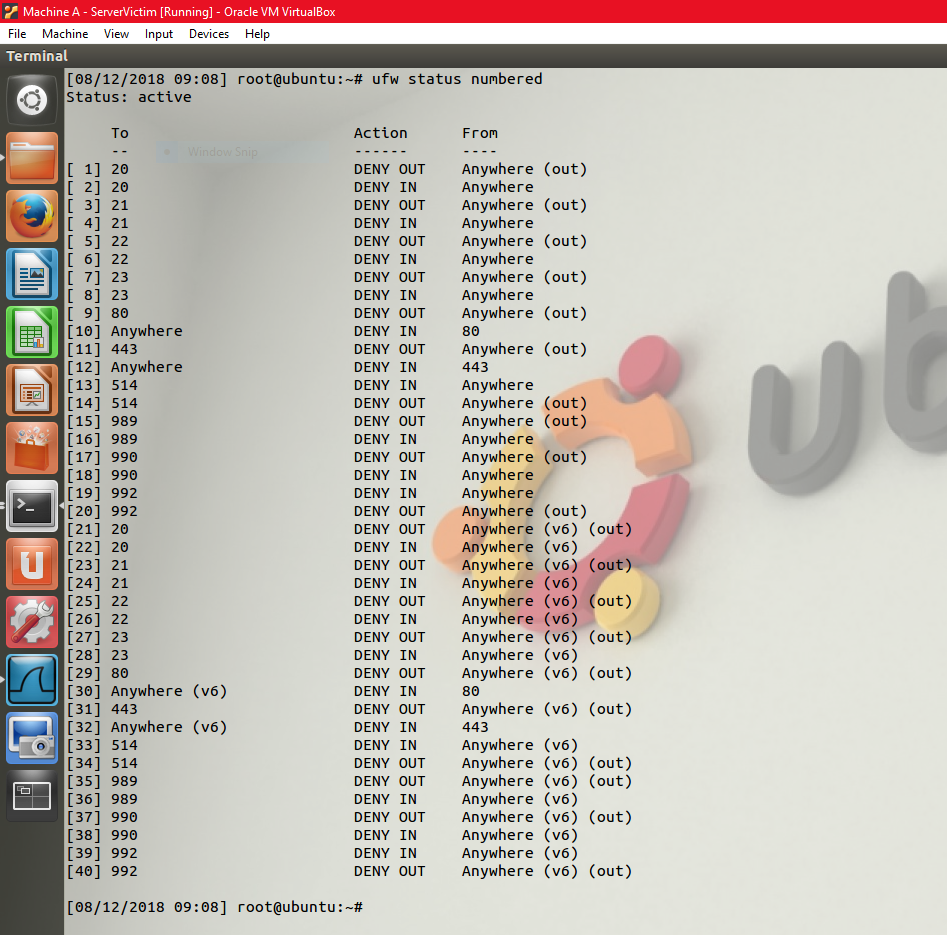
\includegraphics[width=0.7\linewidth]{firewallrule}
		\caption{Active Firewall Blocking on VM1}
		\label{fig:firewallrule}
	\end{figure}
	\fi
	
	\subsection{Task 1: Creating Host-to-Host Tunnel with TUN/TAP}
	TUN/TAP are essential and is widely implemented in modern computing systems. TUN and TAP are virtual network kernel drivers and are implemented entirely by software. TAP (as in network tap) simulates an Ethernet device and operates with layer-2 packets such as Ethernet frames. TUN (as in network TUNnel) simulates a network layer device and operates with layer-3 packets such as IP packets. With TUN/TAP, virtual network interfaces can be created.\\\\A user-space program usually attaches to the TUN/TAP virtual network interface. Packets sent by an operating system via a TUN/TAP network interface are delivered to the user-space program. When packets are sent by the program via a TUN/TAP network interface, the packets are injected into the operating system network stack. On the operating system, the packets appear to originate from an external source through the virtual network interface. \\\\When a program attaches to a TUN/TAP interface, the IP packets that the computer sends to this interface will be piped into the program. IP packets that are sent by the program instead will be piped into the computer, as if they came from the Internet through this virtual network interface. Standard \texttt{read()} and \texttt{write()} function calls can be made to send or receive packets to and from the virtual interface accordingly.\\\\The source code to create a simple TUN/TAP has been provided by Davide Brini\footnote{\url{http://backreference.org/2010/03/26/tuntap-interface-tutorial}} and has been adapted by SEED Labs for this lab. The tutorial for the source code also shows how two computers can be connected using the TUN tunnelling technique. The adapted TUN/TAP code (\texttt{simpletun}) has been attached to \hyperref[ch:AppA]{Appendix A} for reference.
\\\\
	The \texttt{simpletun} program can run as both a client and a server. To run as a client, the \texttt{-c} is used. To run it as a server instead, the \texttt{-s} flag is used. The following list details the requirements to create a tunnel between two computers using the \texttt{simpletun} program.\subsubsection{Setting Up Tunnel Point A}Tunnel point A is set to be the server side of the tunnel, which is on VM1. Once the tunnel between the two systems have been established, there is no difference between client and the server as the concept is only meaningful during the establishment of connection between two systems.\\\\The following command is executed in terminal (with root privileges).
	\begin{verbatim}
	# ./simpletun -i tun0 -s -d
	\end{verbatim}
	\noindent At this point, the virtual network device \texttt{tun0} has been created and the system now has multiple network interfaces. It will not show up if \texttt{ifconfig} is used as the interface is currently not active. Instead, the command \texttt{ip addr show} will list all physical and virtual network interfaces attached to the system regardless of status, as shown in Figure \ref{fig:VirtNet}.
	
	\begin{figure}[H]
		\centering
		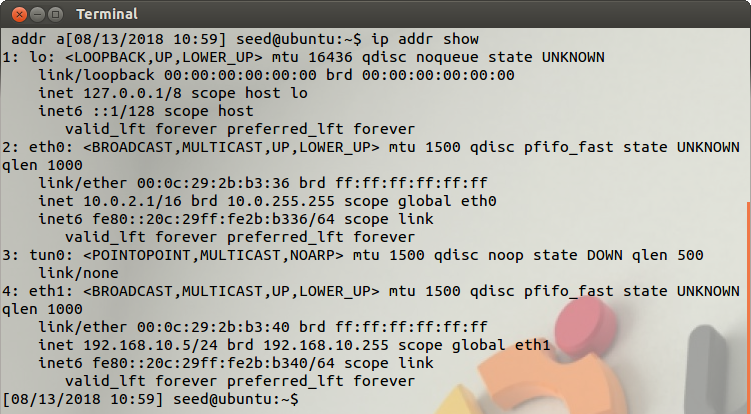
\includegraphics[width=0.9\linewidth]{ipaddr}
		\caption{Virtual Network Details}
		\label{fig:VirtNet}
	\end{figure}
	\noindent The new virtual network device is not fully configured, as evident by the absence of an IP address. The IP address that we will be assigning will be from the reserved IP address space 10.0.0.0/8. It is also important to note that the \texttt{Terminal} window that was used to create the virtual network interface is currently waiting for connections and cannot be used currently. Another window needs to be opened to assign an IP address to the virtual network interface \texttt{tun0}, using the following commands.
	\begin{verbatim}
	# ip addr add 10.0.3.15/24 dev tun0
	# ifconfig tun0 up
	\end{verbatim}
	If \texttt{ifconfig} is used now, it appears as a valid network interface with its configuration displayed.
	
	\begin{figure}[H]
		\centering
		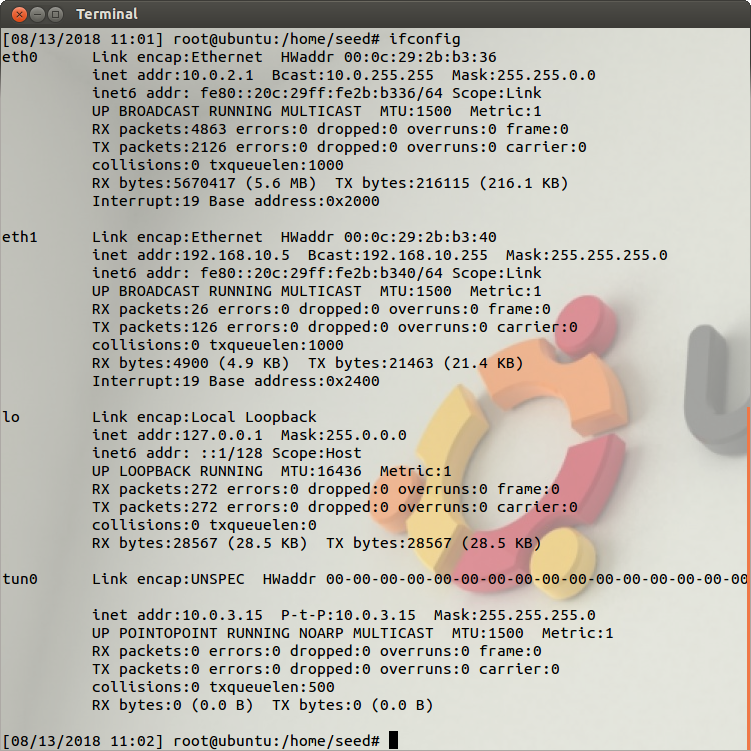
\includegraphics[width=0.7\linewidth]{ifconfig}
		\caption{Valid Network Interfaces}
		\label{fig:ifconfig}
	\end{figure}
	\subsubsection{Setting Up Tunnel Point B}
	Tunnel point B is used as the client side of the tunnel, which is to be on VM2. The setup is similar to VM1. The first command used will connect our client to the server (VM1), which is tunnel point A.
	\begin{verbatim}
	# ./simpletun -i tun0 -c 192.168.10.5 -d
	\end{verbatim}
	Executing the line above will immediately trigger the \texttt{Terminal} window on both VM1 and VM2 to state that the connection between each other has been established. This shows that the configuration is correct.
	\begin{figure}[H]
		\centering
		\begin{subfigure}[H]{0.9\textwidth}
			\centering
			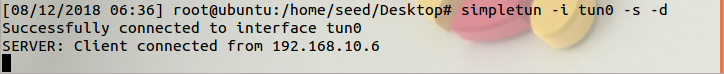
\includegraphics[width=1\linewidth]{server}
			\caption{Server Response}
			\label{fig:serverconn}
		\end{subfigure}
		\\
		\begin{subfigure}{0.9\textwidth}
			\centering
			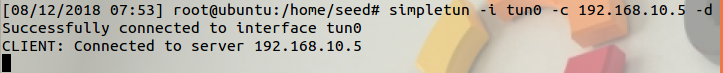
\includegraphics[width=1\linewidth]{client}
			\caption{Client Response}
			\label{fig:clientconn}
		\end{subfigure}
		\caption{Both Systems Connected}
	\end{figure}
	
	\noindent Again, the previous command will prevent any further input in the current window, hence the following commands to initialise the virtual network interface must be done in a separate window.
	\begin{verbatim}
	# ip addr add 10.0.3.16/24 dev tun0
	# ifconfig tun0 up
	\end{verbatim}
	Once it has been executed, the virtual network interface will have all the configurations required to be a functional network adapter.
	\subsubsection{Establishing Routing Path}
	By the previous steps, a tunnel has been established between the two systems. However before it can be used to transmit data, the routing path needs to be set up so that both machines will direct the intended outgoing traffic through the tunnel. The following routing table directs all packs for the 10.0.3.0/24 network through the interface \texttt{tun0}, where the packets will travel through the tunnel. The following must be executed on \textbf{both} VMs:
	\begin{verbatim}
	# route add -net 10.0.3.0 netmask 255.255.255.0 dev tun0
	\end{verbatim}
	\subsubsection{Using The Tunnel}
	Using VM1, we are now able to access VM2 through the \texttt{tun0} adapter. Likewise, VM2 can access VM1 through the \texttt{tun0} adapter as well. The tunnel connection can be tested using the \texttt{ssh} or \texttt{ping} programs.\\\\
	To use \texttt{ssh}, the \texttt{ssh} server must be started first.
	\begin{verbatim}
	$ sudo service ssh start
	\end{verbatim}
	To test the tunnel from VM1:
	\begin{verbatim}
	$ ping 10.0.3.16
	$ ssh 10.0.3.16
	\end{verbatim}
	To test the tunnel from VM2:
	\begin{verbatim}
	$ ping 10.0.3.15
	$ ssh 10.0.3.15
	\end{verbatim}
	\noindent If the tunnel is successful, both \texttt{ssh} and \texttt{ping} will display valid responses from the other system. The figure below shows the packet capture from Wireshark for \texttt{ssh} in both directions is proof that the tunnel works as expected.
	\begin{figure}[H]
		\centering
		\begin{subfigure}[H]{1\textwidth}
			\centering
			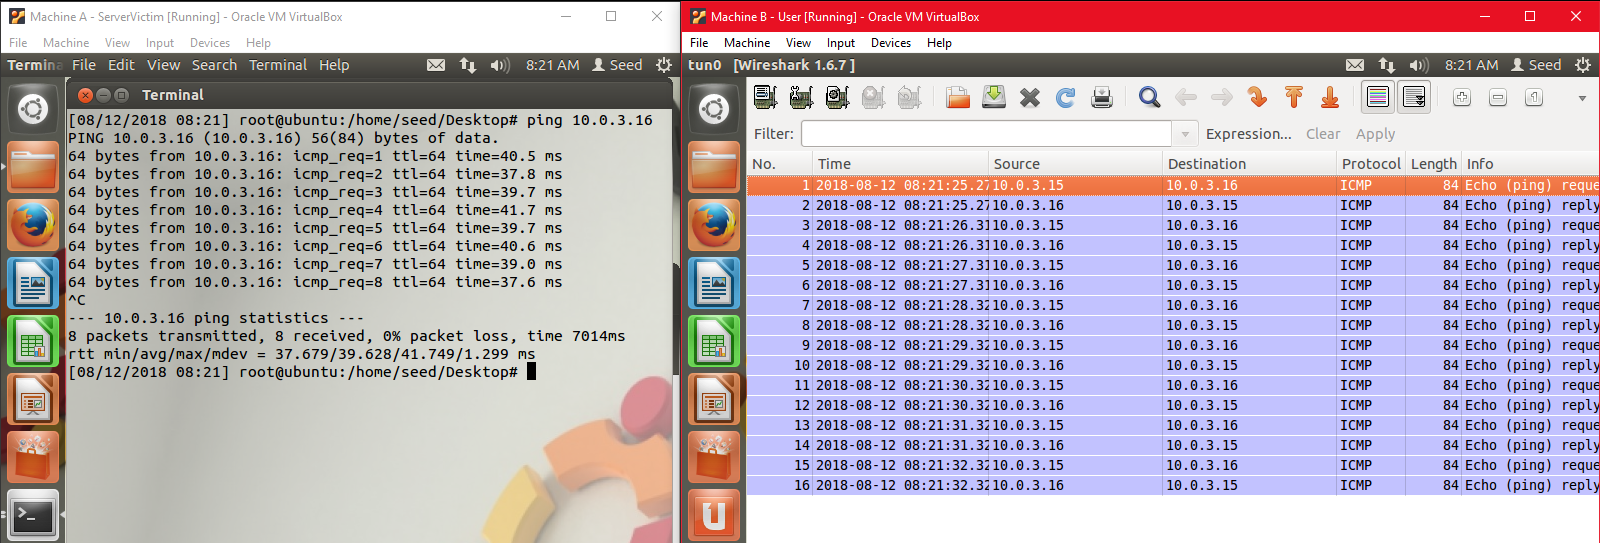
\includegraphics[width=1\linewidth]{wiresharkpingAtoB}
			\caption{\texttt{Ping} from A to B}
			\label{fig:pingAB}
		\end{subfigure}
		\\
		\begin{subfigure}{1\textwidth}
			\centering
			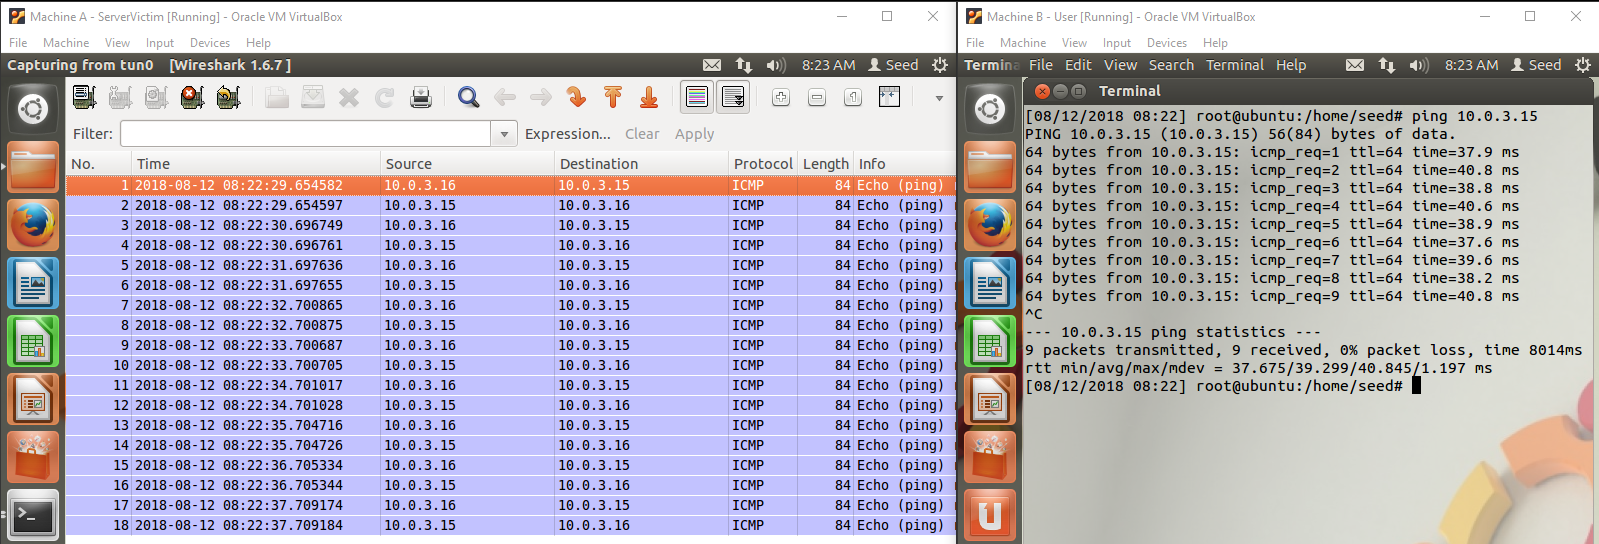
\includegraphics[width=1\linewidth]{wiresharkpingBtoA}
			\caption{\texttt{Ping} from B to A}
			\label{fig:pingBA}
		\end{subfigure}
		\caption{Both Systems Contactable}
	\end{figure}
	\begin{figure}[H]
			\centering
			\begin{subfigure}[H]{0.47\textwidth}
				\centering
				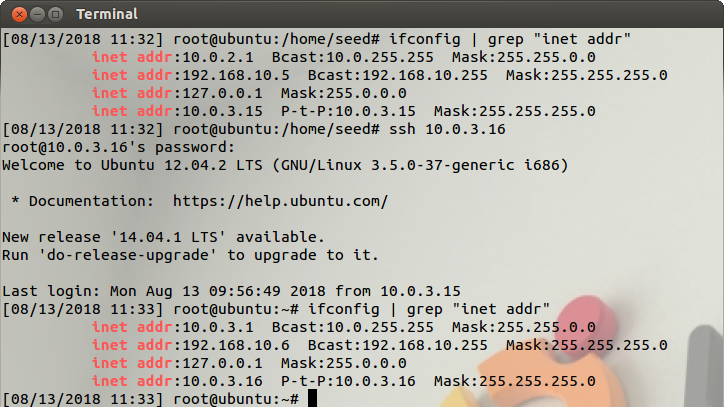
\includegraphics[width=1\linewidth]{sshA2B}
				\caption{\texttt{SSH} from A to B}
				\label{fig:sshAB}
			\end{subfigure}
			~
			\begin{subfigure}{0.47\textwidth}
				\centering
				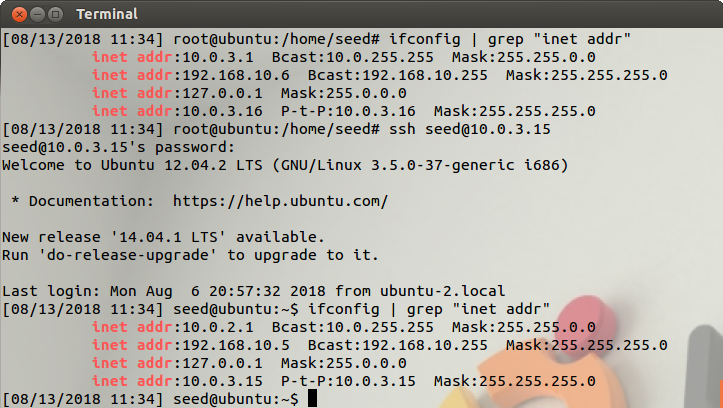
\includegraphics[width=1\linewidth]{sshB2A}
				\caption{\texttt{SSH} from B to A}
				\label{fig:sshBA}
			\end{subfigure}
			\caption{Both Systems Connected}
		\end{figure}
	\noindent Also of interest while the two systems are connected is that data that goes through the tunnel are displayed in the first Terminal window that was opened in VM1 and VM2 (the window that was used to start the \texttt{simpletun} program). Both display the data that was sent to/from the tap interface and the network. It is also noteworthy to notice that the logs on both systems corroborate with the details mentioned in the introduction, which has been summarised into the table below with the corresponding screenshots from the VMs.
	\begin{table}[H]
		\centering
		\begin{tabular}{l|l}
			VM1                                                                                                                     & VM2                                                                                                                     \\ \hline
			\begin{tabular}[c]{@{}l@{}}TAP2NET \textless{}id\textgreater{}: \\ Read x bytes from the tap interface\end{tabular}  & \begin{tabular}[c]{@{}l@{}}NET2TAP \textless{}id\textgreater{}: \\ Read x bytes from the network\end{tabular}        \\ \hline
			\begin{tabular}[c]{@{}l@{}}TAP2NET \textless{}id\textgreater{}: \\ Written x bytes to the network\end{tabular}       & \begin{tabular}[c]{@{}l@{}}NET2TAP \textless{}id\textgreater{}: \\ Written x bytes to the tap interface\end{tabular} \\ \hline
			\begin{tabular}[c]{@{}l@{}}NET2TAP \textless{}id\textgreater{}: \\ Read x bytes from the network\end{tabular}        & \begin{tabular}[c]{@{}l@{}}TAP2NET \textless{}id\textgreater{}: \\ Read x bytes to the tap interface\end{tabular}    \\ \hline
			\begin{tabular}[c]{@{}l@{}}NET2TAP \textless{}id\textgreater{}: \\ Written x bytes to the tap interface\end{tabular} & \begin{tabular}[c]{@{}l@{}}TAP2NET \textless{}id\textgreater{}: \\ Written x bytes to the network\end{tabular}      
		\end{tabular}
		\caption{Differences between logs of both VMs}
		\label{tab:VMLog}
	\end{table}
	\begin{figure}[H]
				\centering
				\begin{subfigure}[H]{0.47\textwidth}
					\centering
					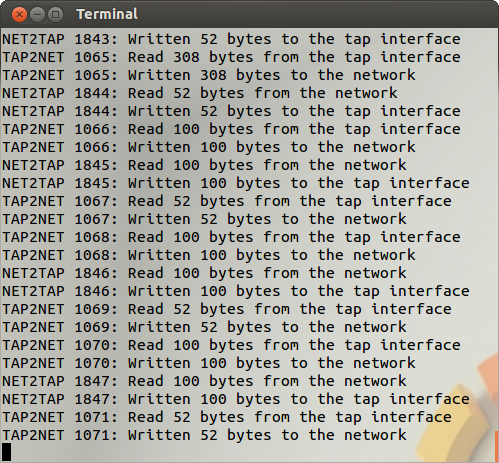
\includegraphics[width=1\linewidth]{VMAlog}
					\caption{Logs from VM1}
					\label{fig:VM1Log}
				\end{subfigure}
				~
				\begin{subfigure}{0.47\textwidth}
					\centering
					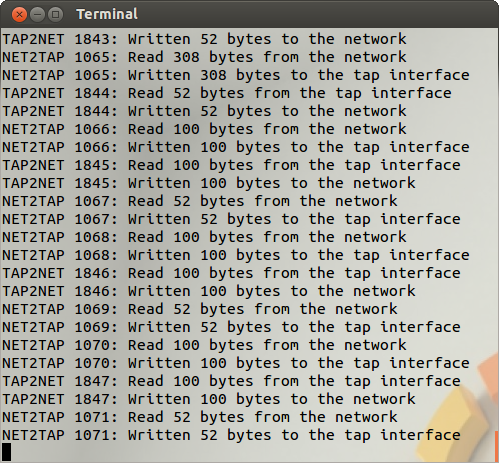
\includegraphics[width=1\linewidth]{VMBlog}
					\caption{Logs from VM2}
					\label{fig:VM2Log}
				\end{subfigure}
				\caption{Logs in Sync}
			\end{figure}
	\noindent To this point, the connection of both VMs using a tunnel has been successful. Figure \ref{fig:H2HTun} is a diagrammatic representation on the current state of the network between the two VMs.
	\begin{figure}[H]
		\centering
		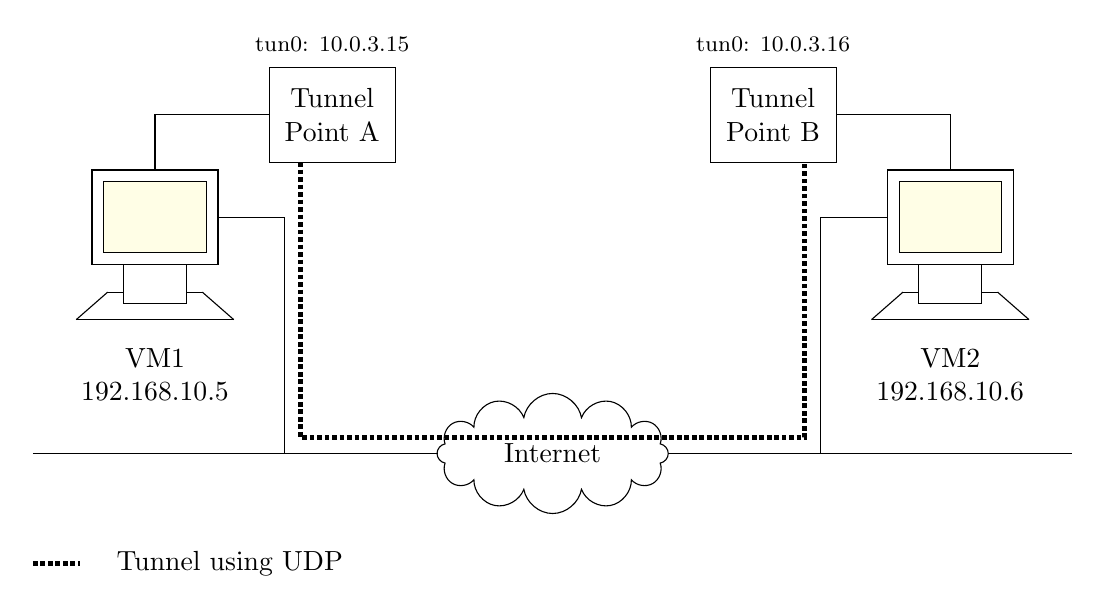
\begin{tikzpicture}			
		\node[cloud, draw,cloud puffs=12,cloud puff arc=160, aspect=3, inner ysep=0.1cm, inner xsep=0.1cm, text width=1.8cm,align=center] at (-0.4,-4.8)  {Internet} ;
		
		\draw[fill=yellow!10] (-6.1,-1.35) rectangle (-4.8,-2.25);
		\draw (-6.25,-1.2) rectangle (-4.65,-2.4);
		\draw (-5.05,-2.4) rectangle (-5.85,-2.9);
		\draw (-6.05,-2.75) -- (-6.45,-3.1);
		\draw (-4.85,-2.75) -- (-4.45,-3.1);
		\draw (-6.45,-3.1) -- (-4.45,-3.1);
		\draw (-6.05,-2.75) -- (-5.85,-2.75);
		\draw (-4.85,-2.75) -- (-5.05,-2.75);
		\draw (-5.45,-3.8) node[text width=3cm,align=center]{VM1\\192.168.10.5};
		
		\draw[fill=yellow!10] (4,-1.35) rectangle (5.3,-2.25);
		\draw (3.85,-1.2) rectangle (5.45,-2.4);
		\draw (5.05,-2.4) rectangle (4.25,-2.9);
		\draw (4.05,-2.75) -- (3.65,-3.1);
		\draw (5.25,-2.75) -- (5.65,-3.1);
		\draw (3.65,-3.1) -- (5.65,-3.1);
		\draw (4.05,-2.75) -- (4.25,-2.75);
		\draw (5.25,-2.75) -- (5.05,-2.75);
		\draw (4.65,-3.8) node[text width=3cm,align=center]{VM2\\192.168.10.6};
		
		\draw (-4.65,-1.8) -- (-3.8,-1.8);
		\draw (3.85,-1.8) -- (3,-1.8);
		\draw (-3.8,-1.8) -- (-3.8,-4.8);
		\draw (3,-1.8) -- (3,-4.8);
		\draw (-7,-4.8)--(-1.86,-4.8);
		\draw (1.07,-4.8)--(6.2,-4.8);
		
		\draw(-5.45,-1.2)-- (-5.45,-0.5) -- (-4,-0.5);
		\draw (-4,-1.1) rectangle node[text width=1.6cm, align=center]{Tunnel\\Point A}(-2.4,0.1);
		\draw (-3.2,0.4) node[align=center]{\footnotesize tun0: 10.0.3.15};
		
		\draw (4.65,-1.2)-- (4.65,-0.5) -- (3.2,-0.5);
		\draw (3.2,-1.1) rectangle node[text width=1.6cm, align=center]{Tunnel\\Point B}(1.6,0.1);
		\draw (2.4,0.4) node[align=center]{\footnotesize tun0: 10.0.3.16};
		
		\draw[densely dotted, line width=0.6mm](-3.6,-1.1) -- (-3.6,-4.6)--(2.8,-4.6)--(2.8,-1.1);
		\draw[densely dotted, line width=0.6mm](-7,-6.2) -- (-6.4,-6.2) node[xshift=1.9cm] {Tunnel using UDP};
		
		\end{tikzpicture}
		\caption{Tunnel Network over Emulated Internet}
		\label{fig:H2HTun}
	\end{figure}
	
	\subsection{Task 2: Creating Host-to-Gateway Tunnel}
	Completing the previous task is insufficient as accessing VM2 through the tunnel is a secondary objective. Instead, the packet sent through the VPN tunnel are to be routed out to the Internet. In other words, VM2 must function as a gateway. This will make our tunnel a host-to-gateway tunnel. As a continuation of the previous task, the following additional tasks must be completed.
	\subsubsection{Setting Up IP Forwarding}
	Unless the system is explicitly configured, a computer will only as a host and not a gateway. To do so, the command below enables IP forwarding, allowing the computer to behave like a gateway.
	\begin{verbatim}
	$ sudo sysctl net.ipv4.ip_forward=1
	\end{verbatim}
	\subsubsection{Getting Around The Limitation of NAT}
	When the destination sends the reply packets back to the machine on the private network, it will reach the NAT first (as the source IP of all outgoing packets are changed to the NAT's external IP address). The NAT will usually replace the destination IP address with the IP address of the original packet and send it to the system to whoever owns the IP address.\\\\Before the NAT sends out the packet, it needs to know the MAC address of the machine that own the IP address 10.0.3.15. To solve the limitation, an extra NAT is created on VM2 so that all packets sent out of VM2 will have VM2's IP address as its source IP. To reach the Internet, the packets will need to go through the NAT adapter that has already been provisioned when the VMs were set-up. The following sets of commands will enable the NAT on VM2.\\\\The first step is to clean all of \texttt{iptables} rules.
	\begin{verbatim}
	$ sudo iptables -F
	$ sudo iptables -t nat -F
	\end{verbatim}
	Next, we need to add a rule on the postrouting position to the NAT adapter, in this instance with \texttt{eth0} (this network adapter may change depending on the interface identified within the VM). The network adapter selected for postrouting must be outward-facing.
	\begin{verbatim}
	$ sudo iptables -t nat -A POSTROUTING -j MASQUERADE -o eth0
	\end{verbatim}
	\subsubsection{Setting Up Firewall}
	The firewall is set up on VM1 to block the access of a target website. Setting up the firewall requires superuser privileges, as with the setup of the VPN tunnel. With reference to the previously completed Firewall lab, popular social media sites Facebook and Twitter are blocked to prevent distractions within organisations.
\\\\
	Setting up the firewall on VM1 invokes an issue where the firewall should not be able to block packets over the virtual network interface or the VPN will not be able to function at all. Therefore, the firewall rule cannot be set before the routing, nor can it be set on the virtual interface.\\\\
	The firewall rule only needs to be set for the physical network interface so it will not affect the virtual network interface. The following \texttt{iptables} command can help to overcome this problem by preventing the packets with the affected IP addresses from going through the physical network adapter \texttt{eth0}.
	\begin{verbatim}
	# iptables -t mangle -A POSTROUTING -d 155.69.7.173/24 -o eth0 -j DROP
	\end{verbatim}
	In the above code, the NTU site (including NTULearn, iNTU etc.) are all blocked as one IP address serves the entire domain. Since NTU is the only site is blocked by the firewall rule, accessing other sites is not an issue. 
	\begin{figure}[H]
	\centering
	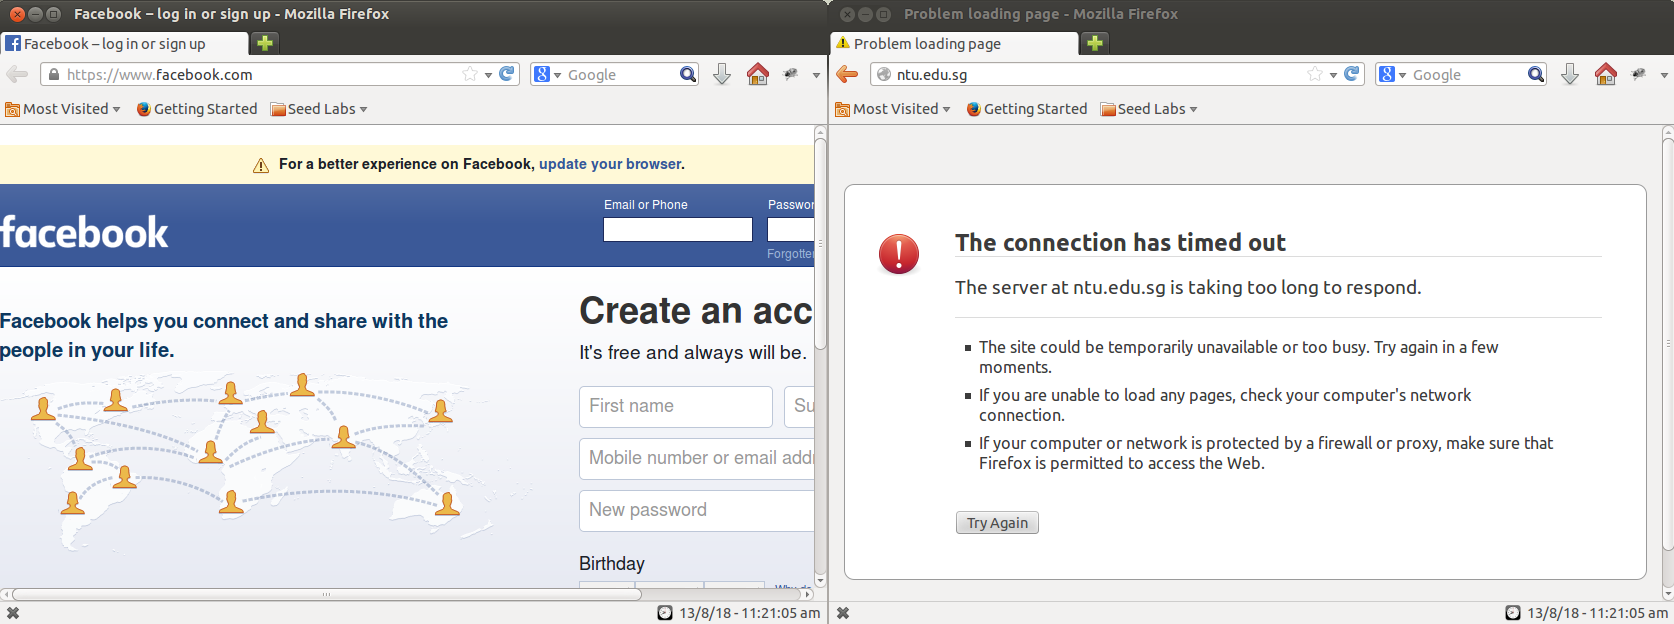
\includegraphics[width=0.9\linewidth]{firewallblock}
	\caption{NTU Site Blocked}
	\label{fig:firewallblock}
	\end{figure}
	\noindent To manually check whether the IP address was properly stored in \texttt{iptables}, the following line of code can be used.
	\begin{verbatim}
	# iptables -L -t mangle --line-numbers
	\end{verbatim}
\begin{figure}[H]
\centering
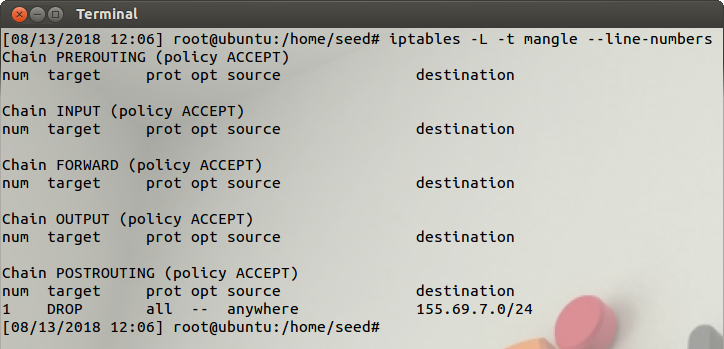
\includegraphics[width=0.7\linewidth]{iptable}
\caption{List of \texttt{mangle} entries}
\label{fig:iptable}
\end{figure}
	\subsubsection{Bypassing Firewall}

To bypass the egress filtering by the firewall, a SSH tunnel is established between the two VMs using the existing VPN tunnel. For web filtering, the dynamic port forwarding (\texttt{-D}) switch can be used as packets will automatically be forwarded to the destinations.
\begin{verbatim}
ssh -D 3000 seed@10.0.3.16
\end{verbatim}
After SSH has been established, the browser must be configured to make use of the dynamic port forwarding mechanism. To do so, we must navigate to the following: \texttt{Edit \textgreater Preferences \textgreater Advanced \textgreater Network \textgreater Settings}. The ``Manual Proxy Configuration'' option must be selected. As we are using SSH, the SOCKS proxy should be used. For the host, it should be \texttt{localhost} with port \texttt{3000}. SOCKS v5 needs to be selected as well. The rest of the options will remain as the default. Figure \ref{fig:proxyconf} is a screenshot of the proxy settings in Firefox.
	\begin{figure}[H]
		\centering
		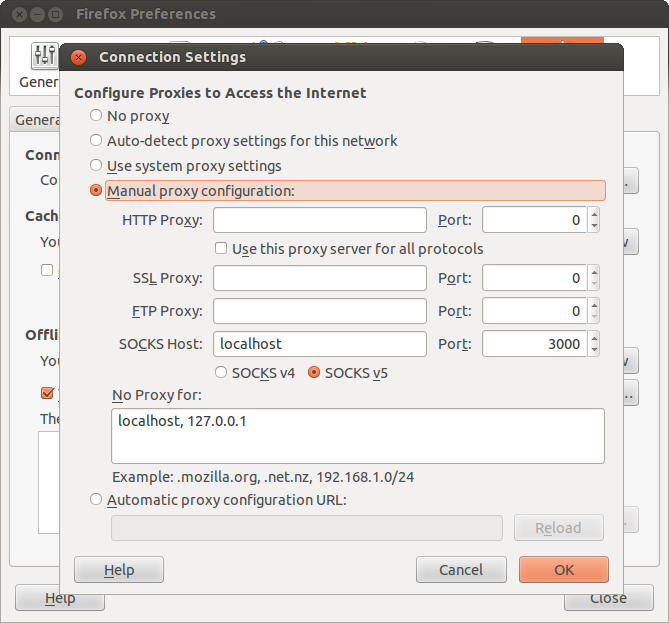
\includegraphics[width=0.7\linewidth]{proxyconf}
		\caption{Proxy Configuration}
		\label{fig:proxyconf}
	\end{figure}
\noindent Once completed, the \textit{Connection Settings} \& \textit{Preferences} windows can be closed and the new settings will take effect immediately. If the proxy has been properly configured, then refreshing the site will allow the page to load up successfully, bypassing the firewall rule.
	\begin{figure}[H]
	\centering
	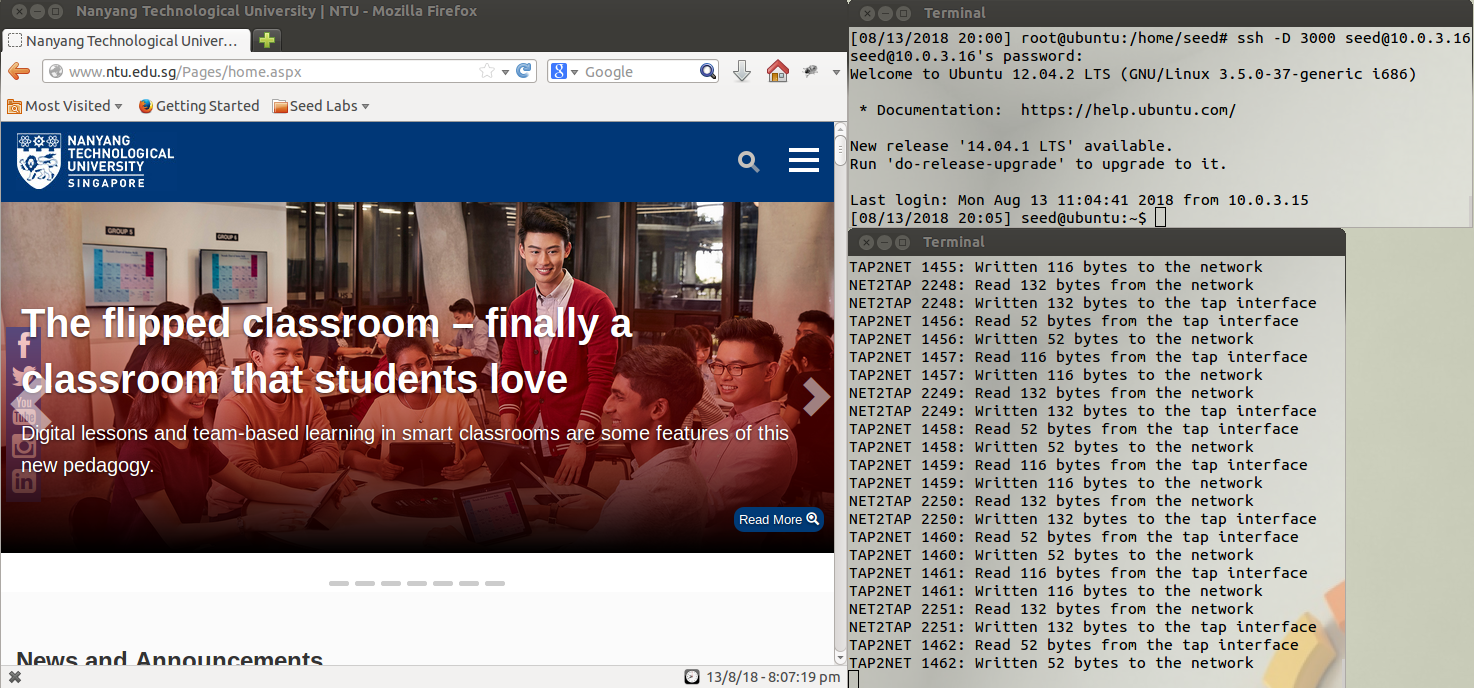
\includegraphics[width=0.9\linewidth]{accessok}
	\caption{Firewall Bypassed For Websites}
	\label{fig:accessok}
	\end{figure}
\noindent To demonstrate how applications can bypass the firewall, \texttt{Telnet} is used as a classic example. To block the \texttt{Telnet} protocol, the packet filtering firewall \texttt{ufw} can be used and it complements \texttt{iptables}. The following lines are executed in superuser privileges.
\begin{verbatim}
# ufw deny out to any port 23
# ufw deny in from any port 23
# ufw disable
# ufw enable
\end{verbatim} 
If there is any attempt to initiate \texttt{Telnet} from VM1, then the \texttt{Telnet} requests will timeout and no connection will be established since all packets are dropped by \texttt{ufw}.
\begin{figure}[H]
\centering
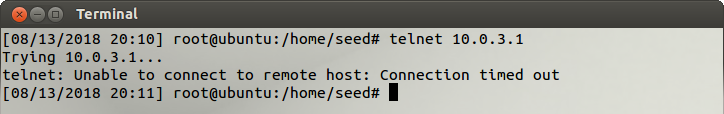
\includegraphics[width=0.9\linewidth]{telnetblock}
\caption{\texttt{Telnet} Timeout}
\label{fig:telnetblock}
\end{figure}
\noindent To use \texttt{Telnet}, the SSH tunnel is made use of again. However, this time static port forwarding is used.
\begin{verbatim}
$ ssh -L 3000:10.0.3.16:23 seed@10.0.3.16
\end{verbatim}
When the SSH tunnel has been established, the \texttt{Telnet} program has to make to use of the static port forwarding rule. To do so, \texttt{Telnet} connects to the source port and \texttt{localhost} to initiate the connection.
\begin{verbatim}
$ telnet localhost 3000
\end{verbatim}
Successful connection through the SSL tunnel will prompt the user login and password of the remote system, in this case VM2. When \texttt{ifconfig | grep "inet addr"} is executed, the IP address that should show up will be for VM2.
\begin{figure}[H]
\centering
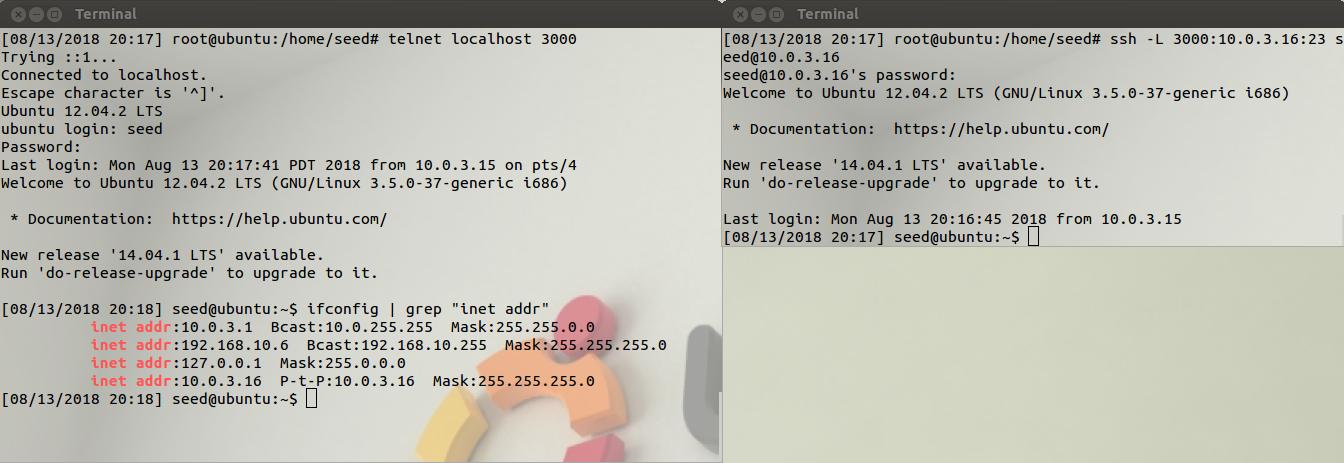
\includegraphics[width=0.9\linewidth]{telnetok}
\caption{Proof of Successful \texttt{Telnet} via \texttt{ifconfig} Checking}
\label{fig:telnetok}
\end{figure}
\noindent
Using Wireshark to analyse the packets between the two VMs, it can be noticed that packets that are from VM1 are sent to \texttt{tun0} with the source and the destination being the host-only network IP address (eth1). This packet is ``repackaged'' and sent through the tunnel by SSH. This is reflected as the source and destination IP of the packet is the IP address of the TUN/TAP that was set in task 1. Again when the data is sent back, the packet headers are modified by the TUN/TAP adapter before it travels through the tunnel.
\begin{figure}[H]
\centering
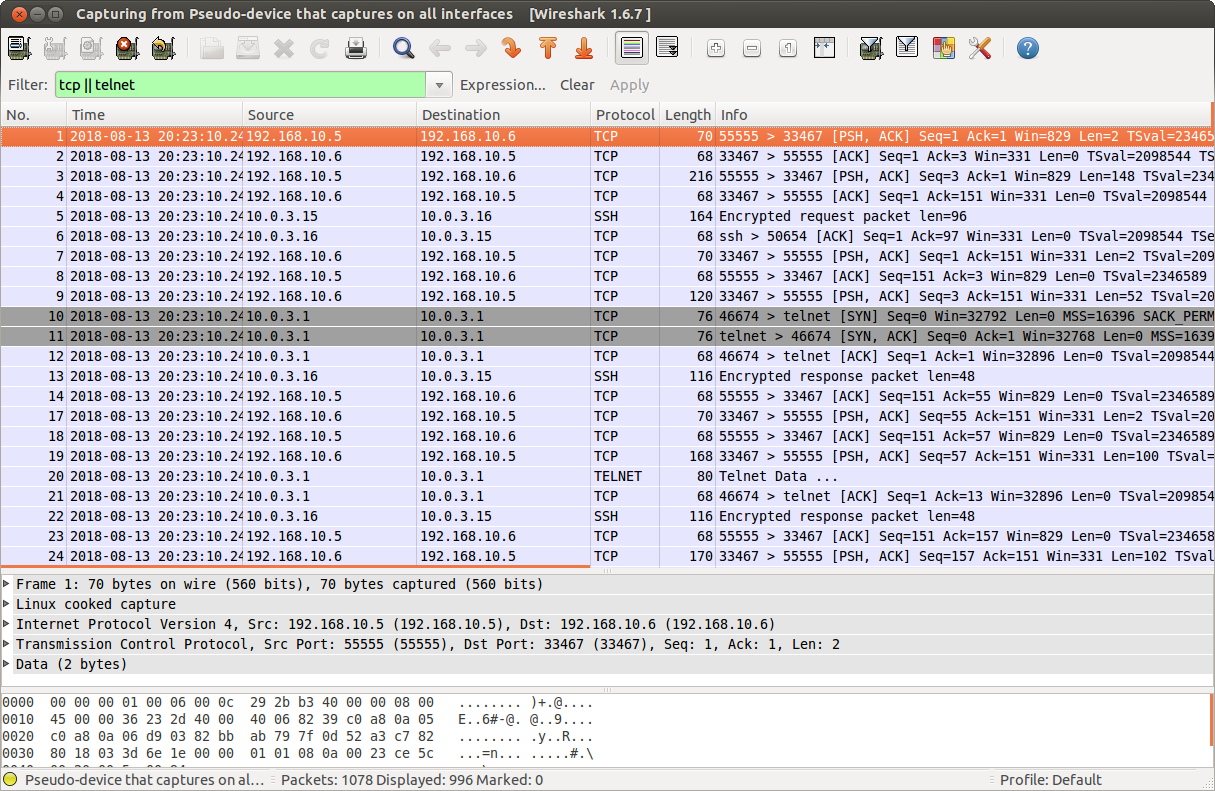
\includegraphics[width=0.9\linewidth]{connectothermac}
\caption{Packet Flow in Wireshark}
\label{fig:connectothermac}
\end{figure}

	\newgeometry{left=1.5cm,top=1cm, bottom=2cm,right=1.5cm}
	\section{Appendix A}
	\label{ch:AppA}
	\begin{minted}[linenos,breaklines]{C}
/**************************************************************************
 * simpletun.c                                                            *
 *                                                                        *
 * A simplistic, simple-minded, naive tunnelling program using tun/tap    *
 * interfaces and TCP. Handles (badly) IPv4 for tun, ARP and IPv4 for     *
 * tap. DO NOT USE THIS PROGRAM FOR SERIOUS PURPOSES.                     *
 *                                                                        *
 * You have been warned.                                                  *
 *                                                                        *
 * (C) 2009 Davide Brini.                                                 *
 *                                                                        *
 * DISCLAIMER AND WARNING: this is all work in progress. The code is      *
 * ugly, the algorithms are naive, error checking and input validation    *
 * are very basic, and of course there can be bugs. If that's not enough, *
 * the program has not been thoroughly tested, so it might even fail at   *
 * the few simple things it should be supposed to do right.               *
 * Needless to say, I take no responsibility whatsoever for what the      *
 * program might do. The program has been written mostly for learning     *
 * purposes, and can be used in the hope that is useful, but everything   *
 * is to be taken "as is" and without any kind of warranty, implicit or   *
 * explicit. See the file LICENSE for further details.                    *
 *************************************************************************/ 

#include <stdio.h>
#include <stdlib.h>
#include <string.h>
#include <unistd.h>
#include <sys/socket.h>
#include <linux/if.h>
#include <linux/if_tun.h>
#include <sys/types.h>
#include <sys/ioctl.h>
#include <sys/stat.h>
#include <fcntl.h>
#include <arpa/inet.h> 
#include <sys/select.h>
#include <sys/time.h>
#include <errno.h>
#include <stdarg.h>

/* buffer for reading from tun/tap interface, must be >= 1500 */
#define BUFSIZE 2000   
#define CLIENT 0
#define SERVER 1
#define PORT 55555

/* some common lengths */
#define IP_HDR_LEN 20
#define ETH_HDR_LEN 14
#define ARP_PKT_LEN 28

int debug;
char *progname;

/**************************************************************************
 * tun_alloc: allocates or reconnects to a tun/tap device. The caller     *
 *            needs to reserve enough space in *dev.                      *
 **************************************************************************/
int tun_alloc(char *dev, int flags) {

  struct ifreq ifr;
  int fd, err;

  if( (fd = open("/dev/net/tun", O_RDWR)) < 0 ) {
    perror("Opening /dev/net/tun");
    return fd;
  }

  memset(&ifr, 0, sizeof(ifr));

  ifr.ifr_flags = flags;

  if (*dev) {
    strncpy(ifr.ifr_name, dev, IFNAMSIZ);
  }

  if( (err = ioctl(fd, TUNSETIFF, (void *)&ifr)) < 0 ) {
    perror("ioctl(TUNSETIFF)");
    close(fd);
    return err;
  }

  strcpy(dev, ifr.ifr_name);

  return fd;
}

/**************************************************************************
 * cread: read routine that checks for errors and exits if an error is    *
 *        returned.                                                       *
 **************************************************************************/
int cread(int fd, char *buf, int n){
  
  int nread;

  if((nread=read(fd, buf, n))<0){
    perror("Reading data");
    exit(1);
  }
  return nread;
}

/**************************************************************************
 * cwrite: write routine that checks for errors and exits if an error is  *
 *         returned.                                                      *
 **************************************************************************/
int cwrite(int fd, char *buf, int n){
  
  int nwrite;

  if((nwrite=write(fd, buf, n))<0){
    perror("Writing data");
    exit(1);
  }
  return nwrite;
}

/**************************************************************************
 * read_n: ensures we read exactly n bytes, and puts those into "buf".    *
 *         (unless EOF, of course)                                        *
 **************************************************************************/
int read_n(int fd, char *buf, int n) {

  int nread, left = n;

  while(left > 0) {
    if ((nread = cread(fd, buf, left))==0){
      return 0 ;      
    }else {
      left -= nread;
      buf += nread;
    }
  }
  return n;  
}

/**************************************************************************
 * do_debug: prints debugging stuff (doh!)                                *
 **************************************************************************/
void do_debug(char *msg, ...){
  
  va_list argp;
  
  if(debug){
	va_start(argp, msg);
	vfprintf(stderr, msg, argp);
	va_end(argp);
  }
}

/**************************************************************************
 * my_err: prints custom error messages on stderr.                        *
 **************************************************************************/
void my_err(char *msg, ...) {

  va_list argp;
  
  va_start(argp, msg);
  vfprintf(stderr, msg, argp);
  va_end(argp);
}

/**************************************************************************
 * usage: prints usage and exits.                                         *
 **************************************************************************/
void usage(void) {
  fprintf(stderr, "Usage:\n");
  fprintf(stderr, "%s -i <ifacename> [-s|-c <serverIP>] [-p <port>] [-u|-a] [-d]\n", progname);
  fprintf(stderr, "%s -h\n", progname);
  fprintf(stderr, "\n");
  fprintf(stderr, "-i <ifacename>: Name of interface to use (mandatory)\n");
  fprintf(stderr, "-s|-c <serverIP>: run in server mode (-s), or specify server address (-c <serverIP>) (mandatory)\n");
  fprintf(stderr, "-p <port>: port to listen on (if run in server mode) or to connect to (in client mode), default 55555\n");
  fprintf(stderr, "-u|-a: use TUN (-u, default) or TAP (-a)\n");
  fprintf(stderr, "-d: outputs debug information while running\n");
  fprintf(stderr, "-h: prints this help text\n");
  exit(1);
}

int main(int argc, char *argv[]) {
  
  int tap_fd, option;
  int flags = IFF_TUN;
  char if_name[IFNAMSIZ] = "";
  int header_len = IP_HDR_LEN;
  int maxfd;
  uint16_t nread, nwrite, plength;
//  uint16_t total_len, ethertype;
  char buffer[BUFSIZE];
  struct sockaddr_in local, remote;
  char remote_ip[16] = "";
  unsigned short int port = PORT;
  int sock_fd, net_fd, optval = 1;
  socklen_t remotelen;
  int cliserv = -1;    /* must be specified on cmd line */
  unsigned long int tap2net = 0, net2tap = 0;

  progname = argv[0];
  
  /* Check command line options */
  while((option = getopt(argc, argv, "i:sc:p:uahd")) > 0){
    switch(option) {
      case 'd':
        debug = 1;
        break;
      case 'h':
        usage();
        break;
      case 'i':
        strncpy(if_name,optarg,IFNAMSIZ-1);
        break;
      case 's':
        cliserv = SERVER;
        break;
      case 'c':
        cliserv = CLIENT;
        strncpy(remote_ip,optarg,15);
        break;
      case 'p':
        port = atoi(optarg);
        break;
      case 'u':
        flags = IFF_TUN;
        break;
      case 'a':
        flags = IFF_TAP;
        header_len = ETH_HDR_LEN;
        break;
      default:
        my_err("Unknown option %c\n", option);
        usage();
    }
  }

  argv += optind;
  argc -= optind;

  if(argc > 0){
    my_err("Too many options!\n");
    usage();
  }

  if(*if_name == '\0'){
    my_err("Must specify interface name!\n");
    usage();
  }else if(cliserv < 0){
    my_err("Must specify client or server mode!\n");
    usage();
  }else if((cliserv == CLIENT)&&(*remote_ip == '\0')){
    my_err("Must specify server address!\n");
    usage();
  }

  /* initialize tun/tap interface */
  if ( (tap_fd = tun_alloc(if_name, flags | IFF_NO_PI)) < 0 ) {
    my_err("Error connecting to tun/tap interface %s!\n", if_name);
    exit(1);
  }

  do_debug("Successfully connected to interface %s\n", if_name);

  if ( (sock_fd = socket(AF_INET, SOCK_STREAM, 0)) < 0) {
    perror("socket()");
    exit(1);
  }

  if(cliserv==CLIENT){
    /* Client, try to connect to server */

    /* assign the destination address */
    memset(&remote, 0, sizeof(remote));
    remote.sin_family = AF_INET;
    remote.sin_addr.s_addr = inet_addr(remote_ip);
    remote.sin_port = htons(port);

    /* connection request */
    if (connect(sock_fd, (struct sockaddr*) &remote, sizeof(remote)) < 0){
      perror("connect()");
      exit(1);
    }

    net_fd = sock_fd;
    do_debug("CLIENT: Connected to server %s\n", inet_ntoa(remote.sin_addr));
    
  } else {
    /* Server, wait for connections */

    /* avoid EADDRINUSE error on bind() */
    if(setsockopt(sock_fd, SOL_SOCKET, SO_REUSEADDR, (char *)&optval, sizeof(optval)) < 0){
      perror("setsockopt()");
      exit(1);
    }
    
    memset(&local, 0, sizeof(local));
    local.sin_family = AF_INET;
    local.sin_addr.s_addr = htonl(INADDR_ANY);
    local.sin_port = htons(port);
    if (bind(sock_fd, (struct sockaddr*) &local, sizeof(local)) < 0){
      perror("bind()");
      exit(1);
    }
    
    if (listen(sock_fd, 5) < 0){
      perror("listen()");
      exit(1);
    }
    
    /* wait for connection request */
    remotelen = sizeof(remote);
    memset(&remote, 0, remotelen);
    if ((net_fd = accept(sock_fd, (struct sockaddr*)&remote, &remotelen)) < 0){
      perror("accept()");
      exit(1);
    }

    do_debug("SERVER: Client connected from %s\n", inet_ntoa(remote.sin_addr));
  }
  
  /* use select() to handle two descriptors at once */
  maxfd = (tap_fd > net_fd)?tap_fd:net_fd;

  while(1) {
    int ret;
    fd_set rd_set;

    FD_ZERO(&rd_set);
    FD_SET(tap_fd, &rd_set); FD_SET(net_fd, &rd_set);

    ret = select(maxfd + 1, &rd_set, NULL, NULL, NULL);

    if (ret < 0 && errno == EINTR){
      continue;
    }

    if (ret < 0) {
      perror("select()");
      exit(1);
    }

    if(FD_ISSET(tap_fd, &rd_set)){
      /* data from tun/tap: just read it and write it to the network */
      
      nread = cread(tap_fd, buffer, BUFSIZE);

      tap2net++;
      do_debug("TAP2NET %lu: Read %d bytes from the tap interface\n", tap2net, nread);

      /* write length + packet */
      plength = htons(nread);
      nwrite = cwrite(net_fd, (char *)&plength, sizeof(plength));
      nwrite = cwrite(net_fd, buffer, nread);
      
      do_debug("TAP2NET %lu: Written %d bytes to the network\n", tap2net, nwrite);
    }

    if(FD_ISSET(net_fd, &rd_set)){
      /* data from the network: read it, and write it to the tun/tap interface. 
       * We need to read the length first, and then the packet */

      /* Read length */      
      nread = read_n(net_fd, (char *)&plength, sizeof(plength));
      if(nread == 0) {
        /* ctrl-c at the other end */
        break;
      }

      net2tap++;

      /* read packet */
      nread = read_n(net_fd, buffer, ntohs(plength));
      do_debug("NET2TAP %lu: Read %d bytes from the network\n", net2tap, nread);

      /* now buffer[] contains a full packet or frame, write it into the tun/tap interface */ 
      nwrite = cwrite(tap_fd, buffer, nread);
      do_debug("NET2TAP %lu: Written %d bytes to the tap interface\n", net2tap, nwrite);
    }
  }
  
  return(0);
}
	\end{minted}
	\restoregeometry
\end{document}